
\section{Dam Break Involving a Dry Area}

The dam break problem involving a dry area was solved analytically by Ritter~\cite{Ritter1892} as well as Stoker~\cite{Stoker1948, Stoker1957}. The analytical solution exhibits a rarefaction fan as a parabolic curve. As water moves, it involves wetting process over the dry area. This is a one-dimensional-type problem. 

The initial condition is
\begin{equation} \label{eq:rdbp}
u(x,0)=0~~, v(x,y)=0, ~~\textrm{and}~~
h(x,0) = \left\{ \begin{array}{ll}
h_1 & \textrm{if $x < x_0$}\\
0 & \textrm{if $x > x_0$}\\
\end{array} \right.
\end{equation}
where $h_1>0$. 

The analytical solution at time $t>0$ is~\cite{Ritter1892, Stoker1948, Stoker1957}
\begin{equation} \label{eq:h_sol_dry}
h(x) = \left\{ \begin{array}{ll}
h_1 & \textrm{if $x \leq -t \sqrt{gh_1}$}\\
h_R=\frac{4}{9g}(\sqrt{gh_1}-\frac{x}{2t})^2 & \textrm{if $-t \sqrt{gh_1} <x \leq 2t\sqrt{gh_1}$}\\
0 & \textrm{if $x \geq 2t\sqrt{gh_1}$}\\
\end{array} \right.
\end{equation}
which is the free surface and
\begin{equation} \label{eq:u_sol_dry}
u(x) = \left\{ \begin{array}{ll}
0 & \textrm{if $x \leq -t \sqrt{gh_1}$}\\
u_R=\frac{2}{3}(\sqrt{gh_1}+\frac{x}{t}) & \textrm{if $-t \sqrt{gh_1} <x \leq 2t\sqrt{gh_1}$}\\
0 & \textrm{if $x \geq 2t\sqrt{gh_1}$}\\
\end{array} \right.
\end{equation}
which is the velocity.



\subsection{Results}
For our test, we consider $x_0=0$ and $h_1=10$ in (\ref{eq:rdbp}).
The following figures show the stage, $x$-momentum, and $x$-velocity at several instants of time. We should see excellent agreement between the analytical and numerical solutions. The wet/dry interface is difficult to resolve and it usually produces large errors.

\begin{figure}[h]
\begin{center}
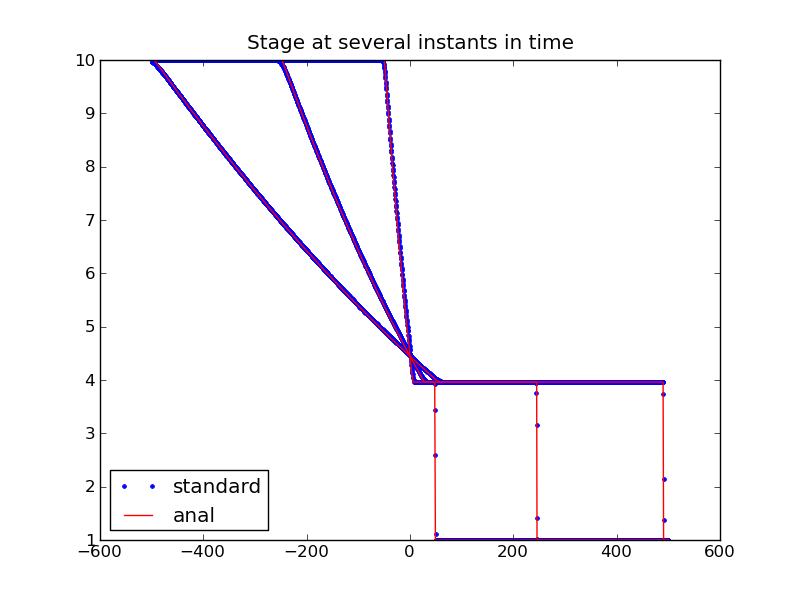
\includegraphics[width=0.8\textwidth]{stage_plot.png}
%\label{fig:db_dry_stage}
\end{center}
\caption{Stage results}
\end{figure}


\begin{figure}[h]
\begin{center}
\includegraphics[width=0.8\textwidth]{xmom_plot.png}
%\label{fig:db_dry_xmom}
\end{center}
\caption{Xmomentum results}
\end{figure}


\begin{figure}[h]
\begin{center}
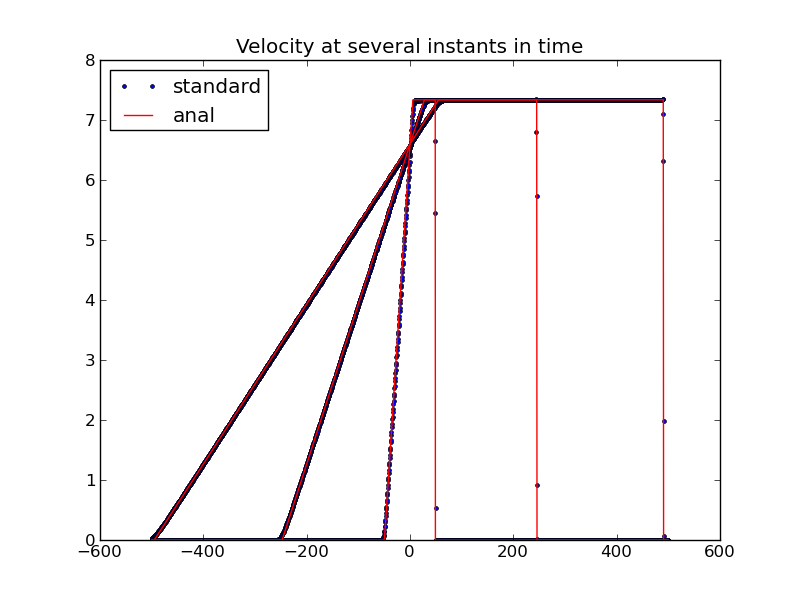
\includegraphics[width=0.8\textwidth]{xvel_plot.png}
%\label{fig:db_dry_xvel}
\end{center}
\caption{Xvelocity results}
\end{figure}


\endinput
